\documentclass[12pt,a4paper,oneside]{article}
\usepackage[utf8]{vietnam}
\usepackage{amsmath}
\usepackage{amsfonts}
\usepackage{amssymb}
\usepackage{graphicx}
\usepackage[left=2cm,right=2cm,top=2cm,bottom=2cm]{geometry}
\usepackage{array}
\usepackage{fancyhdr}
\pagestyle{fancy}
\renewcommand\thesection{\Roman{section}.}
\renewcommand\thesubsection{\arabic{subsection}.}
\fancyhf{}
\rhead{Week 2}
\lhead{Hoàng Quốc Bảo - 20194484}
\rfoot{Trang \thepage}
\begin{document}
\section{Home Assignment 1:}

\subsection{Tên và ý nghĩa của 32 thanh ghi:}

\begin{center}
\begin{tabular}{|>{\raggedright\arraybackslash}p{3cm}|>{\raggedright\arraybackslash}p{4cm}|>{\raggedright\arraybackslash}p{7cm}|}
\hline 
\textbf{Tên thanh ghi} &\textbf{ Số hiệu thanh ghi} & \textbf{Công dụng} \\ 
\hline 
\$zero & 0 & Chứa hằng số = 0 \\ 
\hline 
\$at & 1 & Giá trị tạm thời cho hợp ngữ \\ 
\hline 
\$v0-\$v1 & 2-3 & Các giá trị trả về của thủ tục \\ 
\hline 
\$a0-\$a3 & 4-7 & Các tham số vào của thủ tục \\ 
\hline 
\$t0-\$t7 & 8-15 & Chứa các giá trị tạm thời \\ 
\hline 
\$s0-\$s7 & 16-23 & Lưu các biến \\ 
\hline 
\$t8-\$t9 & 24-25 & Chứa các giá trị tạm thời \\ 
\hline 
\$k0-\$k1 & 26-27 & Các giá trị tạm thời của OS \\ 
\hline 
\$gp & 28 & Con trỏ toàn cục \\ 
\hline 
\$sp & 29 & Con trỏ ngăn xếp \\ 
\hline 
\$fp & 30 & Con trỏ khung \\ 
\hline 
\$ra & 31 & Địa chỉ trả về của toàn cục \\ 
\hline 
\end{tabular} 
\end{center}

\subsection{Các thanh ghi đặc biệt:}

\begin{itemize}
\item PC: là thanh ghi của CPU dùng để giữ địa chỉ của lệnh sẽ được nhận vào
\item HI và LO: Thao tác nhân của MIPS có kết quả chứa trong 2 thanh ghi HI và LO. Bit 0-31 thuộc LO và 32-63 thuộc HI.
\end{itemize}

\subsection{Khuôn dạng của 3 loại lệnh I, J, R:}

\begin{itemize}
\item Lệnh kiểu R:\\
\begin{center}
\begin{tabular}{|c|c|c|c|c|c|}
\hline 
op & rs & rt & rd & shamt & funct \\ 
\hline 
6 bit & 5 bit & 5 bit & 5 bit & 5 bit & 6 bit \\ 
\hline 
\end{tabular} \\
\end{center}
Các trường của lệnh:
	\begin{itemize}
	\item op: Mã thao tác (với lệnh kiểu R, op = 000000)
	\item rs: Số hiệu thanh ghi nguồn thứ nhất
	\item rt: Số hiệu thanh ghi nguồn thứ hai
	\item rd: Số hiệu thanh ghi đích
	\item shamt (shift amount): số bit được dịch, chỉ dùng cho lệnh dịch bit, với các lệnh khác shamt = 00000
	\item funct: mã hàm -> mã hoá cho thao tác cụ thể
	\end{itemize}
\item Lệnh kiểu I:\\
\begin{center}
\begin{tabular}{|c|c|c|c|}
\hline 
op & rs & rt & imm \\ 
\hline 
6 bit & 5 bit & 5 bit & 16 bit \\ 
\hline 
\end{tabular} \\
\end{center}
Dùng cho các lệnh số học/logic với toán hạng tức thì và các lệnh load/store.\\
Với lệnh addi:
	\begin{itemize}
	\item rs: Số hiệu thanh ghi nguồn
	\item rt: Số hiệu thanh ghi đích
	\end{itemize}
Với lệnh lw, sw:
	\begin{itemize}
	\item rs: Số hiệu thanh ghi cơ sở
	\item rt: Số hiệu thanh ghi đích (lw) hoặc số hiệu thanh ghi nguồn (sw)	
	\end{itemize}
\item Lệnh kiểu J:
\begin{center}
\begin{tabular}{|c|c|}
\hline 
op & address \\ 
\hline 
6 bit & 26 bit \\ 
\hline 
\end{tabular} \\
\end{center}
Toán hạng 26 địa chỉ, được sử dụng cho các lệnh nhảy.

\end{itemize}
\pagebreak
\section{Assignment 1: Lệnh gán số 16 bit}
	\textbf{Mã nguồn:}
	
	\begin{center}
    		\begin{figure}[htp]
    		\begin{center}
     	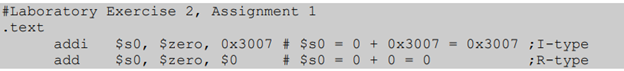
\includegraphics[scale=1]{image/1}
    		\end{center}
    		\label{refhinh1}
    		\end{figure}
	\end{center}
	
	\subsection{Quan sát cửa sổ Register:}
	Giá trị của các thanh ghi ở trong bảng sau\\
	\begin{center}
	 \begin{tabular}{|l|l|l|>{\raggedright\arraybackslash}p{8cm}|}
	\hline 
	Lần chạy & \$s0 & \$pc & Giải thích \\ 
	\hline 
	0 & 0x00000000 & 0x00400000 & Đây là các giá trị mặc định của \$s0 và \$pc \\ 
	\hline 
	1 & 0x00003007 & 0x00400004 & Sau khi chạy lệnh addi, thanh ghi \$s0 có số hiệu thanh ghi là 16 sẽ được gán giá trị tương ứng là 0x00003007. Sau khi lệnh được nhận vào, nội dung \$pc tự động tăng 4 byte để trỏ đến lệnh kế tiếp. (0x00400000 -> 0x00400004) \\ 
	\hline 
	2 & 0x00000000 & 0x00400008 & Sau khi chạy lệnh add, thanh ghi \$s0 sẽ có giá trị là 0x00000000 (\$s0 = \$0 + \$0). Sau khi lệnh được nhận vào, nội dung \$pc tự động tăng 4 byte để trỏ đến lệnh kế tiếp. (0x00400004 -> 0x00400008) \\ 
	\hline 
	\end{tabular}
	 \end{center} 
	\subsection{Quan sát cửa sổ Text Segment:\\}
	\begin{center}
	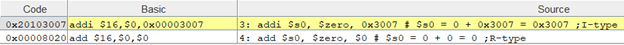
\includegraphics[scale=1]{image/2}
	\end{center}
	
	\begin{itemize}
	\item Khuôn dạng lệnh thứ nhất (lệnh kiểu I)
	\begin{center}
	 \begin{tabular}{|c|c|c|c|}
	\hline 
	op & rs & rt & imm \\ 
	\hline 
	001000 & 00000 & 10000 & 0011000000000111 \\ 
	\hline 
	\multicolumn{4}{|l|}{Hexa: 0x20103007} \\ 
	\hline 
	\end{tabular}
	 \end{center} 
	\item Khuôn dạng lệnh thứ hai (Lệnh kiểu R)
	\begin{center}
	\begin{tabular}{|c|c|c|c|c|c|}
	\hline 
	op & rs & rt & rd & shamt & funct \\ 
	\hline 
	000000 & 00000 & 00000 & 10000 & 00000 & 100000 \\ 
	\hline 
	\multicolumn{6}{|l|}{Hexa: 0x00008020} \\ 
	\hline 
	\end{tabular} 
	\end{center}
	Ta thấy mã máy của các lệnh trên đúng với tập lệnh đã quy định
	\end{itemize}
	
	\subsection{Sửa lại lệnh: \quad\quad\quad\quad 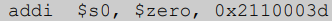
\includegraphics[scale=1]{image/3}}
		Ta quan sát thấy ở cửa sổ Text Segment, xuất hiện thêm 2 lệnh lui và ori\\ \begin{center}
		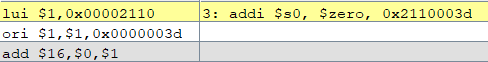
\includegraphics[scale=1]{image/4}
		\end{center}
\textbf{Giải thích}: Do hằng số được addi vào \$s0 là hằng số 32 bit nên chương trình tự động chuyển thành lệnh lui và ori dể xử lý hằng số 32 bit. Copy 16 bit cao của hằng số 32 bit vào nửa bên trái rt (lui), Xoá 16 bit bên phải của rt về 0 , đưa 16 bit thấp của hằng số 32-bit vào nửa bên phải rt. (ori)
\pagebreak
\section{Assignment 2: Lệnh gán số 32-bit}
	\textbf{Mã nguồn:}
	\begin{center}
	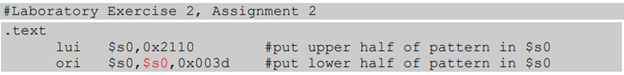
\includegraphics[scale=1]{image/5}
	\end{center}
	\subsection{Quan sát cửa sổ Register:}
		\begin{center}
		\begin{tabular}{|l|l|l|>{\raggedright\arraybackslash}p{8cm}|}
		\hline 
		Lần chạy & \$0 & \$pc & Giải thích \\ 
		\hline 
		0 & 0x00000000 & 0x00400000 & Đây là các giá trị mặc định của \$s0 và \$pc \\ 
		\hline 
		1 & 0x21100000 & 0x00400004 & Lệnh lui copy 16 bit vào nửa bên trái của \$s0. Sau khi lệnh được nhận vào, nội dung \$pc tự động tăng 4 byte để trỏ đến lệnh kế tiếp. (0x00400000 -> 0x00400004) \\ 
		\hline 
		2 & 0x2110003d & 0x00400008 & Lệnh ori đưa 16 bit vào nửa bên phải \$s0. Sau khi lệnh được nhận vào, nội dung \$pc tự động tăng 4 byte để trỏ đến lệnh kế tiếp. (0x00400004 -> 0x00400008) \\ 
		\hline 
		\end{tabular} 
		\end{center}
	\subsection{Quan sát cửa sổ Data Segment:}
	Ta thấy:
	\begin{center}
	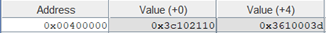
\includegraphics[scale=1.5]{image/6}
	\end{center}
	Mã máy tương ứng: 
	\begin{center}
	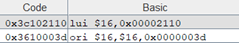
\includegraphics[scale=1.5]{image/7}
	\end{center}
	Vậy địa chỉ vùng lệnh 0x00400000 tương ứng với câu lệnh thứ nhất (lui), địa chỉ vùng lệnh 0x00400004 tương ứng với câu lệnh thứ hai (ori).
\pagebreak
\section{Assignment 3: Lệnh gán (giả lệnh):}
	\textbf{Mã nguồn:}
		\begin{center}
		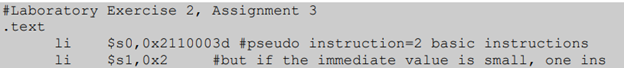
\includegraphics[scale=1]{image/8}
		\end{center}
	\subsection{Quan sát cửa sổ Text Segment}
		Sau khi biên dịch thì ta thấy 2 câu lệnh gán (li) được chuyển thành 3 câu lệnh (lui, ori, addiu)
		\begin{center}
		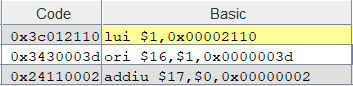
\includegraphics[scale=1]{image/9}
		\end{center}
		\textbf{Giải thích:}
			\begin{itemize}
			\item Ở câu lệnh thứ nhất là lệnh gán 32 bit -> chương trình sẽ tự động tách thành 2 lệnh lui và ori. Lệnh lui copy 16 bit cao của hằng số 32 bit vào nửa bên trái của \$1 (2110), lệnh ori copy 16 bit thấp của hằng số 32 bit vào nửa bên trái của \$1 (003d).
			\item Ở câu lệnh thứ hai là lệnh gán 16 bit -> chương trình thực hiện phép gán li bằng câu lệnh addiu như bình thường. (addiu khác với addi ở chỗ sẽ không báo lỗi khi tràn số).
			\end{itemize}
\pagebreak
\section{Assignment 4: tính biểu thức 2x + y = ?}
	\textbf{Mã nguồn:}
		\begin{center}
		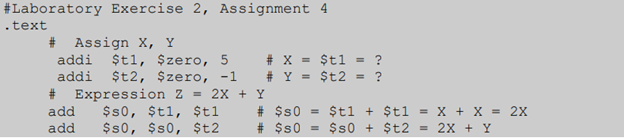
\includegraphics[scale=1]{image/10}
		\end{center}
	\subsection{Quan sát cửa sổ Register:}
		\begin{center}
		\begin{tabular}{|l|l|l|l|l|}
		\hline 
		Lần chạy & \$0 & \$t1 & \$t2 & Giải thích	 \\ 
		\hline 
		0 & 0x00000000 & 0x00000000 & 0x00000000 & Đây là các giá trị khởi đầu \\ 
		\hline 
		1 & 0x00000000 & 0x00000005 & 0x00000000 & Gán giá trị 5 cho \$t1 \\ 
		\hline 
		2 & 0x00000000 & 0x00000005 & 0xffffffff & Gán giá trị -1 cho \$t2 \\ 
		\hline 
		3 & 0x0000000a & 0x00000005 & 0xffffffff & \$s0 = \$t1 + \$t1 = 5 + 5 = 10 \\ 
		\hline 
		4 & 0x00000009 & 0x00000005 & 0xffffffff & \$s0 = \$s0 + \$s2 = 10 – 1 = 9 \\ 
		\hline 
		\end{tabular} 
		\end{center}
		\quad Sau khi kết thúc chương trình, kết quả chính xác (2x – y = 2*5 + (-1) = 9) 
	\subsection{Quan sát cửa sổ Text Segment}
		\begin{itemize}
		
			\item Ta thấy hợp ngữ và mã máy có điểm tương đồng thông qua khuôn mẫu của kiểu lệnh I
		\begin{center}
			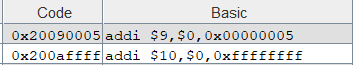
\includegraphics[scale=1]{image/11}
		\end{center}
			\item Chuyển mã máy của lệnh add sang hệ 2:
			\begin{itemize}
				\item Lệnh thứ nhất \quad \quad 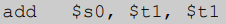
\includegraphics[scale=1]{image/12}
				\begin{center}
	\begin{tabular}{|c|c|c|c|c|c|}
	\hline 
	op & rs & rt & rd & shamt & funct \\ 
	\hline 
	000000 & 01001 & 01001 & 10000 & 00000 & 100000 \\ 
	\hline 
	\multicolumn{6}{|l|}{Hexa: 0x01298020} \\ 
	\hline 
	\end{tabular} 
	\end{center}
		\item Lệnh thứ hai \quad \quad 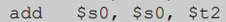
\includegraphics[scale=1]{image/13}
				\begin{center}
	\begin{tabular}{|c|c|c|c|c|c|}
	\hline 
	op & rs & rt & rd & shamt & funct \\ 
	\hline 
	000000 & 10000 & 01010 & 10000 & 00000 & 100000 \\ 
	\hline 
	\multicolumn{6}{|l|}{Hexa: 0x020a8020} \\ 
	\hline 
	\end{tabular} 
	\end{center}
\end{itemize}			 
Ta thấy mã máy của lệnh add sau khi chuyển đúng với khuôn mẫu của kiểu lệnh R
		\end{itemize}
		\pagebreak
\section{Assignment 5: Phép nhân}
	\textbf{Mã nguồn:}
		\begin{center}
		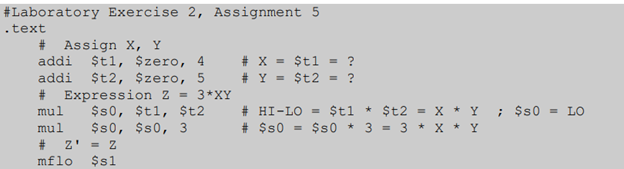
\includegraphics[scale=1]{image/14}
		\end{center}
	\subsection{Quan sát cửa sổ Text Segment:}
	Sau khi biên dịch mã máy, chương trình đã tự động tách 5 lệnh thành 6 lệnh.
		\begin{center}
		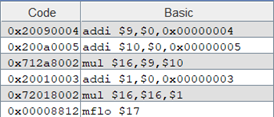
\includegraphics[scale=1.2]{image/15}
		\end{center}
	\subsection{Quan sát cửa sổ Register}
	\begin{center}
	\begin{small}
	 \begin{tabular}{|c|c|c|c|c|c|c|c|}
	\hline 
	Lần chạy & \$s0 & \$s1 & \$t1 & \$t2 & Hi & Lo & \$at \\ 
	\hline 
	0 & 0x00000000 & 0x00000000 & 0x00000000 & 0x00000000 & 0x00000000 & 0x00000000 & 0x00000000 \\ 
	\hline 
	1 & 0x00000000 & 0x00000000 & 0x00000004 & 0x00000000 & 0x00000000 & 0x00000000 & 0x00000000 \\ 
	\hline 
	2 & 0x00000000 & 0x00000000 & 0x00000004 & 0x00000005 & 0x00000000 & 0x00000000 & 0x00000000 \\ 
	\hline 
	3 & 0x00000014 & 0x00000000 & 0x00000004 & 0x00000005 & 0x00000000 & 0x00000014 & 0x00000000 \\ 
	\hline 
	4 & 0x00000014 & 0x00000000 & 0x00000004 & 0x00000005 & 0x00000000 & 0x00000014 & 0x00000003 \\ 
	\hline 
	5 & 0x0000003c & 0x00000000 & 0x00000004 & 0x00000005 & 0x00000000 & 0x0000003c & 0x00000003 \\ 
	\hline 
	6 & 0x0000003c & 0x0000003c & 0x00000004 & 0x00000005 & 0x00000000 & 0x0000003c & 0x00000003 \\ 
	\hline 
	\end{tabular}
	 \end{small} 
	\end{center}
	\textbf{Giải thích:\\}
	\begin{center}
	\begin{tabular}{|c|>{\raggedright\arraybackslash}p{11cm}|}
	\hline 
	Lần chạy & Giải thích \\ 
	\hline 
	0 & Đây là các giá trị khởi đầu \\ 
	\hline 
	1 & Gán giá trị 4 cho \$t1 \\
	\hline 
	2 & Gán giá trị 5 cho \$t2 \\ 
	\hline 
	3 & Gán giá trị \$s0 = \$t1 * \$t2. Do kết quả là 32 bit nên thanh ghi Lo sẽ được cập nhật kết quả này. (Lo = 20) \\ 
	\hline 
	4 & Phép nhân \$0 = \$s0 * 3 đã được tách thành 2 lệnh ở lần chạy 4 và 5. Ở lần chạy 4, thực hiện phép gán \$at = 3  \\ 
	\hline 
	5 & Ở lần chạy 5, thực hiện nhân \$s0 = \$s0 * \$at = \$s0 * 3 \linebreak = 0x0000003c = 60. Thanh ghi Lo cũng cập nhật kết quả này. \\ 
	\hline 
	6 & Lấy giá trị của thanh ghi Lo ghi vào \$s1. (\$s1 = 60) \\ 
	\hline 
	\end{tabular} 
	\end{center}
	Sau khi kết thúc chương trình, ta thấy kết quả thu được là chính xác. (\$s0 = 3 * X * Y \linebreak  = 3 * 4 * 5 = 60 = 0x0000003c)
\section{Assignment 6: Tạo biến và truy cập biến}
	\textbf{Mã nguồn:}
	\begin{center}
	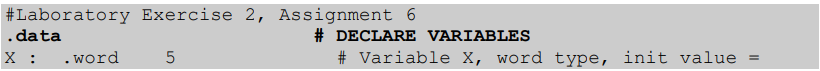
\includegraphics[scale=0.8]{image/16}
	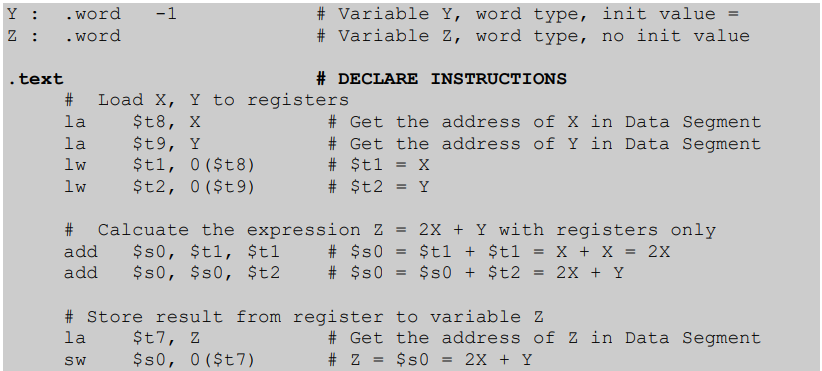
\includegraphics[scale=0.8]{image/17}
	\end{center}
	\subsection{Quan sát cửa sổ Text Segment}
	\begin{center}
	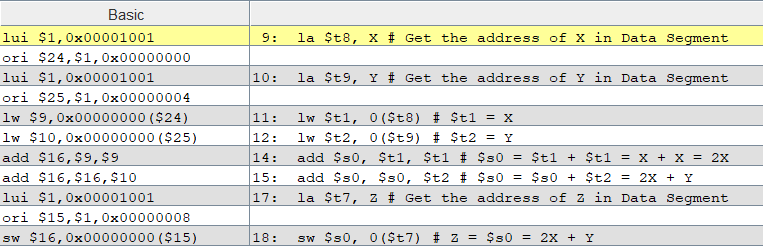
\includegraphics[scale=0.8]{image/18}
	\end{center}
	\quad Lệnh la được tách ra thành 2 lệnh lui và ori. Lệnh lui copy địa chỉ 16 bit bên trái của biến vào thanh ghi tạm thời \$at. Lệnh ori copy địa chỉ 16 bit bên phải của biến, kết hợp với 16 bit bên trái của thanh ghi \$at, ghi vào thanh ghi đích.
	\subsection{Quan sát cửa sổ Label}
	\begin{itemize}
	\item So sánh với hằng số khi biên dịch
		\begin{itemize}
	\item Hằng số khi quan sát trên cửa sổ Label: \begin{center}
	 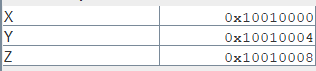
\includegraphics[scale=0.8]{image/19}
	\end{center}
	\item Hằng số khi biên dịch lệnh la thành mã máy: \begin{center}
	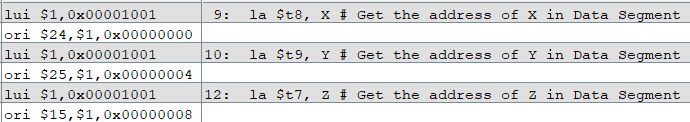
\includegraphics[scale=0.8]{image/20}
	\end{center}
	\end{itemize}
	Ta thấy giá trị hằng số trên cửa sổ Label giống với hằng số khi biên dịch lệnh la thành mã máy.
	\item Click đúp vào các giá trị X, Y, Z
	\begin{itemize}
	\item Giá trị của X:\quad\quad 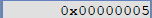
\includegraphics[scale=0.8]{image/21}
	\item Giá trị của Y:\quad\quad 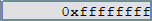
\includegraphics[scale=0.8]{image/22}
	\item Giá trị của Z:\quad\quad 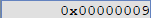
\includegraphics[scale=0.8]{image/23}
	\end{itemize}
	Ta thấy giá trị của các biến biến X, Y, Z trong bộ nhớ ở cửa số Data Segment giống với các giá trị đã khai báo ban đầu.
	\end{itemize}
	\subsection{Quan sát cửa sổ Register:}
	\begin{itemize}
	\item Quan sát sự thay đổi của các thanh ghi qua từng lần chạy
	\item Xác định vai trò của lệnh lw và sw
	\begin{itemize}
	\item Lệnh lw: \textbf{nạp} word dữ liệu 32-bit từ bộ nhớ đưa vào thanh ghi, thông qua địa chỉ sơ sở và hằng số dịch chuyển địa chỉ.
	\item Lệnh sw: \textbf{lưu} word dữ liệu 32-bit từ thanh ghi ra bộ nhớ, thông qua địa chỉ sơ sở và hằng số dịch chuyển địa chỉ.
	\end{itemize}
	\end{itemize}
	\subsection{Tìm hiểu thêm về lệnh lb, sb}
	\begin{itemize}
	\item Lệnh lb:
	\begin{itemize}
	\item Nạp 1 byte hoặc 2 byte (halfword) từ bộ nhớ vào bên phải thanh ghi đích rt 
	\item Phần còn lại của thanh ghi rt được mở rộng có dấu thành 32-bit (Sign-extended)
	\end{itemize}
	\item Lệnh sb:\\Chỉ lưu byte/halfword bên phải thanh ghi rt ra bộ nhớ .
	\end{itemize}
\end{document}